\subsubsection{Opis przypadków użycia - części}

Poniżej przedstawiono przypadki użycia związane z zarządzaniem częściami. W większości przypadków aktorem jest pracownik sklepu uprawniony do zarządzania częściami. Wyjątkiem jest lista części dostępnych do kupienia, którą może także wyświetlić klient.

\begin{figure}[h!]
    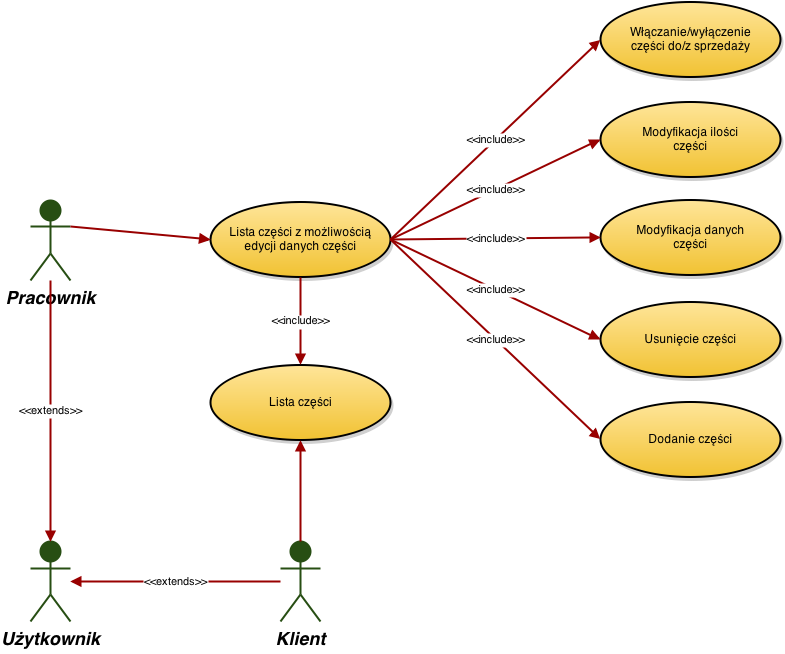
\includegraphics[width=\textwidth,
    height=0.5\textheight]{graphics/UseCase/Czesci/UseCaseDiagram.png}
  \caption{Diagram przypadków użycia związanych z zarządzaniem częściami}
\end{figure}

\begin{figure}[h!]
    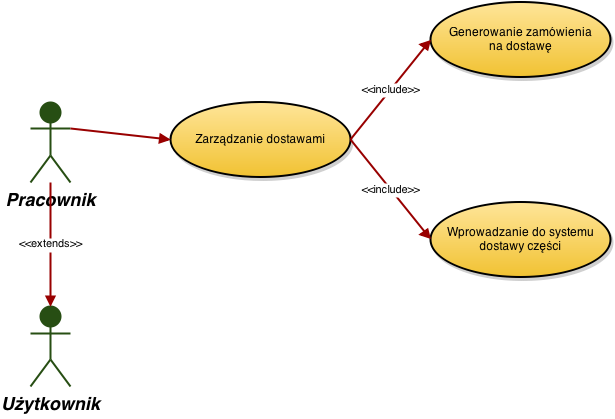
\includegraphics[width=\textwidth,
    height=0.5\textheight]{graphics/UseCase/Czesci/DostawyUseCase.png}
  \caption{Diagram przypadków użycia związanych z zarządzaniem dostawami}
\end{figure}

\newpage
\begin{enumerate}
   \item Wyświetlanie listy części - scenariusz główny \\
 
 Opis słowny - jest to podstawowy przypadek użycia jeśli chodzi o zarządzanie częściami, gdyż zapewnia on funkcjonalność prezentacji wszystkich dostępnych w sklepie części. Jest to funkcjonalność używana zarówno przez klientów sklepu (w celu przeglądania asortymentu sklepu), jak i przez pracowników (w celu zarządzania częściami). W przypadku gdy użytkownik posiada odpowiednie uprawnienia (pracownik magazynu), lista części udostępnia także funkcjonalności zarządzania częściami (modyfikacja, usuwanie, itd. - dokładnie opisane poniżej).
 
 \begin{longtable}{|p{5cm}|p{7cm}|}
 	\hline
	\textbf{Aktor} & Klient lub pracownik \\
	\hline
	\textbf{Warunki początkowe} & Brak \\
	\hline
	\textbf{Opis przebiegu interakcji} & Wybór prezentacji listy części na stronie głównej sklepu \\
	\hline
	\textbf{Sytuacje wyjątkowe} & Ustawienie kryteriów filtrowania, posiadanie przez użytkownika specjalnych uprawnień do zarządania częściami \\
	\hline
	\textbf{Warunki końcowe} & Wyświetlenie listy dostępnych części \\
	\hline
 \end{longtable}
 
  \item Wyświetlanie listy części - scenariusz główny \label{lista-czesci} \\
  \begin{tabularx}{\linewidth}{ c X}
  Aktor: & Klient lub pracownik \\
  \end{tabularx}
   \begin{enumerate}
    \item Użytkownik (nie posiadający specjalnych uprawnień) uruchamia stronę internetową sklepu i wybiera opcję wyświetlenia listy części.
    \item System prezentuje listę dostępnych dla użytkownika części (możliwych do kupienia), posortowaną alfabetycznie, z podziałem wyników na strony (10 wartości na stronie, z możliwością zmiany tej liczby przez użytkownika na 25, 50 i 100).
  \end{enumerate}
  
  \item Wyświetlanie listy części - scenariusz alternatywny - ustawiono kryteria filtrowania \\
  \begin{tabularx}{\linewidth}{ c X}
  Aktor: & Klient lub pracownik \\
  \end{tabularx}
   \begin{enumerate}
     \item Krok 1 scenariusza głównego.
     \item Użytkownik ustawia żądane przez siebie kryteria filtrowania. Filtrować można po kodzie części, jej nazwie, opisie i cenie.
     \item System prezentuje odfiltrowaną listę części. Sposób prezentacji taki sam jak w scenariuszu głównym, kroku 2.
   \end{enumerate} 
   
   \item Wyświetlanie listy części - scenariusz alternatywny - użytkownik posiada specjalne uprawnienia do zarządzania częściami \\
   \begin{tabularx}{\linewidth}{ c X}
	Aktor: & Pracownik \\
  	\end{tabularx}   
  	\begin{enumerate}
     \item Krok 1 scenariusza głównego.
  	  \item System prezentuje listę części w taki sam sposób jak dla kroku 2 scenariusza głównego, ale dodatkowo przy każdym elemencie listy dostępne są przyciski, umożliwiające pracownikowi edycję danych części lub usunięcie jej z systemu. Na tym ekranie widoczny jest także przycisk umożliwiający dodanie nowego typu części do systemu. Działanie tych przycisków opisane jest w kolejnych przypadkach użycia. Dodatkowo na liście widoczne są także części ukryte (niewidoczne dla kupujących).
  	\end{enumerate}	
  	
\begin{figure}[h!]
    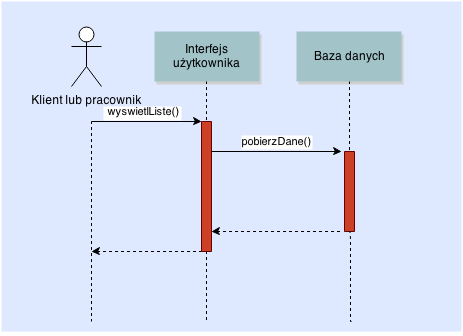
\includegraphics[width=\textwidth,
    height=0.5\textheight]{graphics/UseCase/Czesci/ListaCzesciSD.png}
  \caption{Diagram sekwencji dla przypadku użycia Lista części - scenariusz główny}
\end{figure}
   \item Dodanie części - scenariusz główny \\
 
 Opis słowny - ten przypadek użycia opisuje funkcjonalność dodawania nowych typów części, czyli takich które nie są jeszcze zarejestrowane w systemie. Obejmuje to sytuację, gdy np. sklep decyduje się na wprowadzenie nowego asortymentu do sprzedaży.
 
 \begin{longtable}{|p{5cm}|p{7cm}|}
 	\hline
	\textbf{Aktor} & Pracownik \\
	\hline
	\textbf{Warunki początkowe} & Posiadanie konta z uprawnieniami umożliwiającymi zarządzanie częściami, zalogowanie się do systemu \\
	\hline
	\textbf{Opis przebiegu interakcji} & Wybór prezentacji listy części na stronie głównej sklepu, wybranie opcji dodania nowej części, uzupełnienie danych, zatwierdzenie operacji \\
	\hline
	\textbf{Sytuacje wyjątkowe} & Dodawana część już istnieje, podanie błędnych danych nowej części \\
	\hline
	\textbf{Warunki końcowe} & Dodanie do systemu nowego typu części \\
	\hline
 \end{longtable}
 
  \item Dodanie części - scenariusz główny \\
  \begin{tabularx}{\linewidth}{ c X}
  Aktor: & Pracownik \\
  \end{tabularx}
   \begin{enumerate}
    \item Scenariusz ``Wyświetlanie listy części - scenariusz alternatywny - użytkownik posiada specjalne uprawnienia do zarządzania częściami''. \label{dodanie-czesci-poczatek}
    \item Pracownik wybiera opcję dodania nowej części.
    \item System prezentuje pracownikowi formatkę dodania nowej części, z możliwością wypełnienia następujących atrybutów części:
    \begin{enumerate}
      \item Kod części (generowany automatycznie, z możliwością edycji przez pracownika)
      \item Nazwa części
      \item Opis części
      \item Zdjęcie części (w jedym z popularnych formatów graficznych, takich jak JPG, PNG czy GIF)
      \item Cena jednostkowa części
      \item Widoczność części dla klientów (czy klienci będą mogli zobaczyć część na liście części możliwych do kupienia)
      \item Minimalna liczba sztuk w magazynie
    \end{enumerate}
    \item Pracownik uzupełnia wymagane pola i zatwierdza operację. \label{dodanie-czesci-zatwierdzenie}
    \item System dodaje część do bazy danych i informuje użytkownika o zakończeniu operacji.
  \end{enumerate}
  
  \item Dodanie części - scenariusz alternatywny - dodawana część już istnieje \\
  \begin{tabularx}{\linewidth}{ c X}
  Aktor: & Pracownik \\
  \end{tabularx}
   \begin{enumerate}
    \item Kroki \ref{dodanie-czesci-poczatek} do \ref{dodanie-czesci-zatwierdzenie} scenariusza głównego.
    \item System sprawdza czy istnieje już część o podanym kodzie. Jeśli tak, wyświetla komunikat o błędzie i anuluje operację. Jeśli nie, to powrót do scenariusza głównego.
  \end{enumerate}
  
  \item Dodanie części - scenariusz alternatywny - podanie błędnych danych nowej części \\
  \begin{tabularx}{\linewidth}{ c X}
  Aktor: & Pracownik \\
  \end{tabularx}
   \begin{enumerate}
    \item Kroki \ref{dodanie-czesci-poczatek} do \ref{dodanie-czesci-zatwierdzenie} scenariusza głównego.
    \item System sprawdza czy podane przez użytkownika dane są poprawne, czyli:
    \begin{enumerate}
      \item Czy wszystkie pola oprócz opisu i zdjęcia są wypełnione
      \item Czy podana cena nie jest ujemna
      \item Czy podana minimalna liczba sztuk na magazynie nie jest ujemna
    \end{enumerate}
    \item W przypadku niepoprawności wprowadzonych danych, system wyświetla stosowny komunikat błędu i anuluje operację. W przeciwnym przypadku powrót do scenariusza głównego.
  \end{enumerate}
  	
\begin{figure}[h!]
    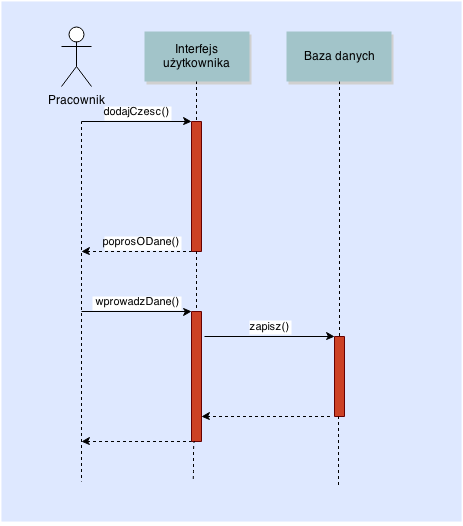
\includegraphics[width=\textwidth,
    height=0.7\textheight]{graphics/UseCase/Czesci/DodanieCzesciSD.png}
  \caption{Diagram sekwencji dla przypadku użycia Dodanie części - scenariusz główny}
\end{figure}
   \item Usunięcie części - scenariusz główny \\
 
 Opis słowny - ten przypadek użycia opisuje funkcjonalność usuwania istniejących typów części. Obejmuje to sytuację, gdy np. sklep decyduje się na usunięcie starego asortymentu ze sprzedaży.
 
 \begin{longtable}{|p{5cm}|p{7cm}|}
 	\hline
	\textbf{Aktor} & Pracownik \\
	\hline
	\textbf{Warunki początkowe} & Posiadanie konta z uprawnieniami umożliwiającymi zarządzanie częściami, zalogowanie się do systemu \\
	\hline
	\textbf{Opis przebiegu interakcji} & Wybór prezentacji listy części na stronie głównej sklepu, wybranie opcji usunięcia konkretnej części, zatwierdzenie operacji \\
	\hline
	\textbf{Sytuacje wyjątkowe} & Istnieje niezerowa liczba części tego typu w magazynie \\
	\hline
	\textbf{Warunki końcowe} & Usunięcie z systemu wybranego typu części \\
	\hline
 \end{longtable}
 
  \item Usunięcie części - scenariusz główny \\
  \begin{tabularx}{\linewidth}{ c X}
  Aktor: & Pracownik \\
  \end{tabularx}
   \begin{enumerate}
    \item Scenariusz ``Wyświetlanie listy części - scenariusz alternatywny - użytkownik posiada specjalne uprawnienia do zarządzania częściami''. \label{usuniecie-czesci-poczatek}
    \item Pracownik wyszukuje na liście część którą chce usunąć i wybiera przycisk usunięcia. \label{usuniecie-czesci-wybor}
    \item System prosi użytkonika o potwierdzenie operacji.
    \item Pracownik zatwierdza operację.
    \item System usuwa część z bazy danych i informuje użytkownika o zakończeniu operacji.
  \end{enumerate}
  
  \item Dodanie części - scenariusz alternatywny - istnieje niezerowa liczba części tego typu w magazynie \\
  \begin{tabularx}{\linewidth}{ c X}
  Aktor: & Pracownik \\
  \end{tabularx}
   \begin{enumerate}
    \item Kroki \ref{usuniecie-czesci-poczatek} do \ref{usuniecie-czesci-wybor} scenariusza głównego.
    \item System sprawdza czy w magazynie znajdują się części danego typu. Jeśli tak (na magazynie znajduje się co najmniej 1 sztuka danego typu części), informuje o tym pracownika w formie ostrzeżenia.
    \item Powrót do scenariusza głównego.
  \end{enumerate}
  	
\begin{figure}[h!]
    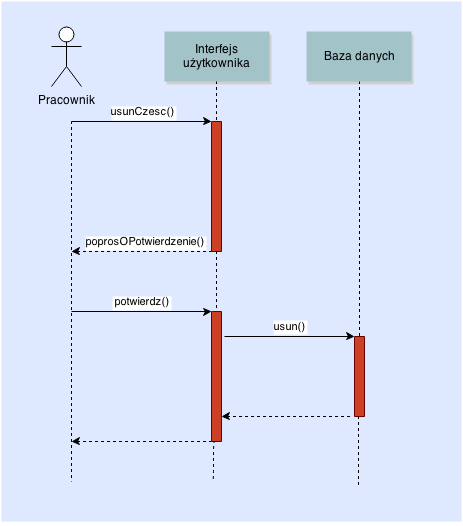
\includegraphics[width=\textwidth,
    height=0.7\textheight]{graphics/UseCase/Czesci/UsuniecieCzesciSD.png}
  \caption{Diagram sekwencji dla przypadku użycia Usunięcie części - scenariusz główny}
\end{figure}
   \item Modyfikacja danych części - scenariusz główny \\
 
 Opis słowny - ten przypadek użycia opisuje funkcjonalność modyfikacji danych istniejących typów części. Obejmuje to sytuację, gdy np. cena danej części musi zostać zmieniona.
 
 \begin{longtable}{|p{5cm}|p{7cm}|}
 	\hline
	\textbf{Aktor} & Pracownik \\
	\hline
	\textbf{Warunki początkowe} & Posiadanie konta z uprawnieniami umożliwiającymi zarządzanie częściami, zalogowanie się do systemu \\
	\hline
	\textbf{Opis przebiegu interakcji} & Wybór prezentacji listy części na stronie głównej sklepu, wybranie opcji modyfikacji konkretnej części, wprowadzenie danych, zatwierdzenie operacji \\
	\hline
	\textbf{Sytuacje wyjątkowe} & Podanie błędnych danych przy modyfikacji części \\
	\hline
	\textbf{Warunki końcowe} & Modyfikacja danych wybranej części \\
	\hline
 \end{longtable}
 
  \item Modyfikacja danych części - scenariusz główny \\
  \begin{tabularx}{\linewidth}{ c X}
  Aktor: & Pracownik \\
  \end{tabularx}
   \begin{enumerate}
    \item Scenariusz ``Wyświetlanie listy części - scenariusz alternatywny - użytkownik posiada specjalne uprawnienia do zarządzania częściami''. \label{modyfikacja-czesci-poczatek}
    \item Pracownik wyszukuje na liście część którą chce zmodyfikować i wybiera przycisk modyfikacji.
    \item System prezentuje pracownikowi formatkę taką jak dla dodania nowej części, ale wypełnioną danymi modyfikowanej części, z możliwością ich edycji. Dodatkowo, istnieje możliwość edycji liczby części wybranego typu, znajdujących się aktualnie w magazynie.
    \item Pracownik modyfikuje wybrane pola i zatwierdza operację. \label{modyfikacja-czesci-zatwierdzenie}
    \item System modyfikuje część w bazie danych i informuje użytkownika o zakończeniu operacji.
  \end{enumerate}
  
  \item Modyfikacja danych części - scenariusz alternatywny - podanie błędnych danych przy modyfikacji części \\
  \begin{tabularx}{\linewidth}{ c X}
  Aktor: & Pracownik \\
  \end{tabularx}
   \begin{enumerate}
    \item Kroki \ref{modyfikacja-czesci-poczatek} do \ref{modyfikacja-czesci-zatwierdzenie} scenariusza głównego.
    \item System sprawdza czy zmodyfikowane przez użytkownika dane są poprawne, czyli:
    \begin{enumerate}
      \item Czy wszystkie pola oprócz opisu i zdjęcia są wypełnione
      \item Czy podana cena nie jest ujemna
      \item Czy podana minimalna liczba sztuk na magazynie nie jest ujemna
      \item Czy podana aktualna liczba sztuk na magazynie nie jest ujemna
    \end{enumerate}
    \item W przypadku niepoprawności wprowadzonych danych, system wyświetla stosowny komunikat błędu i anuluje operację. W przeciwnym przypadku powrót do scenariusza głównego.
  \end{enumerate}
  	
\begin{figure}[h!]
    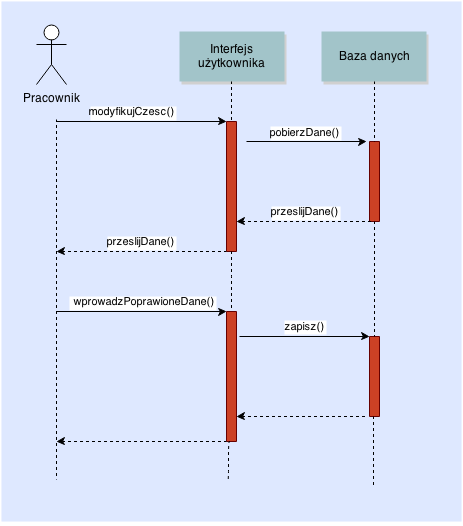
\includegraphics[width=\textwidth,
    height=0.7\textheight]{graphics/UseCase/Czesci/ModyfikacjaCzesciSD.png}
  \caption{Diagram sekwencji dla przypadku użycia Modyfikacja części - scenariusz główny}
\end{figure}
   \item Generowanie zamówienia na dostawę części - scenariusz główny \\
 
 Opis słowny - ten przypadek użycia opisuje funkcjonalność generowania zamówienia na dostawę części, których ilość w magazynie spadnie poniżej zadanego poziomu, ustawianego oddzielnie dla każdej części. Jest to funkcjonalność bardzo ułatwiająca pracę pracownikom magazynu, którzy dbają o zaopatrzenie sklepu, ponieważ po ustawieniu minimalnej liczby sztuk towaru, system sam dba o to, żeby poziom ten zawsze był utrzymany, zwalniając z tego obowiązku pracowników. Skutkuje to także mniejszą liczbą pomyłek przy zamawianiu dostaw.
 
 \begin{longtable}{|p{5cm}|p{7cm}|}
 	\hline
	\textbf{Aktor} & Pracownik \\
	\hline
	\textbf{Warunki początkowe} & Posiadanie konta z uprawnieniami umożliwiającymi zarządzanie częściami, zalogowanie się do systemu \\
	\hline
	\textbf{Opis przebiegu interakcji} & Wybór opcji zarządzania dostawami na stronie głównej sklepu, wybranie opcji generowania zamówienia na dostawę, wprowadzenie danych, zatwierdzenie operacji \\
	\hline
	\textbf{Sytuacje wyjątkowe} & Brak \\
	\hline
	\textbf{Warunki końcowe} & Utworzenie dokumentu, zawierającego listę części które należy zamówić przy najbliższej dostawie \\
	\hline
 \end{longtable}
 
\begin{figure}[h!]
    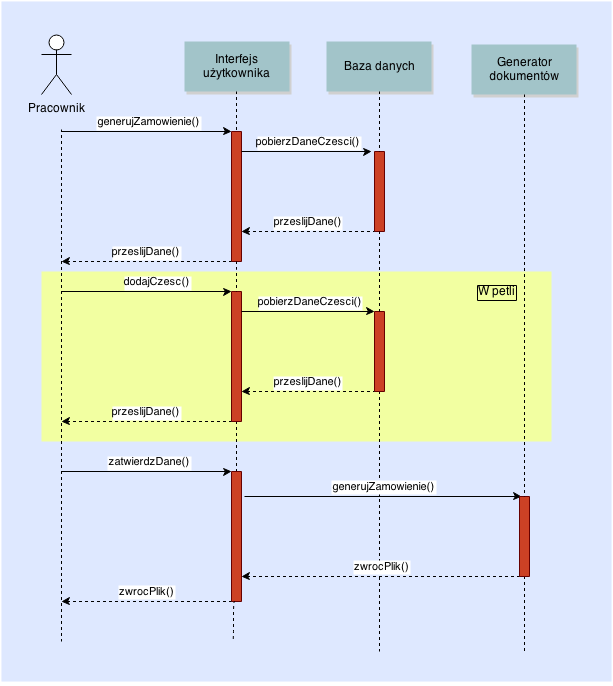
\includegraphics[width=\textwidth,
    height=0.7\textheight]{graphics/UseCase/Czesci/GenerowanieZamowieniaSD.png}
  \caption{Diagram sekwencji dla przypadku użycia Generowanie zamówienia na dostawę części - scenariusz główny}
\end{figure}
  \item Generowanie zamówienia na dostawę części - scenariusz główny \\
  \begin{tabularx}{\linewidth}{ c X}
  Aktor: & Pracownik \\
  \end{tabularx}
   \begin{enumerate}
    \item Pracownik otwiera stronę internetową sklepu, loguje się na swoje konto i wybiera opcję zarządzania dostawami.
    \item System prezentuje widok generowania zamówienia na dostawę, umożliwiający:
    \begin{enumerate}
      \item Dodanie typu części do zamówienia.
      \item Usunięcie wcześniej wprowadzonego typu części z zamówienia.
      \item Prezentację listy już wprowadzonych części.
    \end{enumerate}
    \item System początkowo wypełnia listę tymi częściami, których ilość w magazynie spadła poniżej zadanego minimalnego poziomu. Części dodawane są w minimalnej ilości wystarczającej do tego, aby poziom ten został osiągnięty.
    \item Pracownik dodaje nowe części według następującego schematu:
    \begin{enumerate}
      \item Pracownik wybiera przycisk umożliwiający dodanie typu części do zamówienia.
      \item System prezentuje listę części z możliwością wyszukiwania tak jak w przypadku użycia ``Wyświetlanie listy części''.
      \item Pracownik wybiera żądany typ części i wpisuje ilość sztuk (liczba naturalna większa od zera), jaka ma zostać dodana do zamówienia.
      \item Pracownik zatwierdza operację.
      \item Powrót do widoku generowania zamówienia.
    \end{enumerate}
    \item Po wprowadzeniu wszystkich informacji o zamówieniu, pracownik zatwierdza operację.
    \item System prosi pracownika o potwierdzenie zamiaru wygenerowania zamówienia.
    \item W przypadku potwierdzenia zamiaru przez pracownika, system generuje plik PDF z zamówieniem na dostawę.
    \item Pracownik pobiera plik i wysyła go do dostawcy.
  \end{enumerate}


\end{enumerate}